%----------------------------------------------------------------------
\begin{frame}{Cohorts where all are exposed}
When there is no comparison group we may ask:\\
Do mortality rates in cohort differ from those of an
\textbf{external} population, for example:

Rates from:
\begin{itemize}
\item Occupational cohorts
\item Patient cohorts
\end{itemize}
compared with reference rates obtained from:
\begin{itemize}
\item Population statistics (mortality rates)
\item Hospital registers (disease rates)
% \item Cancer registers
\end{itemize}
\end{frame}

%----------------------------------------------------------------------
\begin{frame}{Cohort rates vs. population rates: RSR}
  \begin{itemize}
  \item \textbf{Additive:} $\lambda(a) = \delta(a) + \lambda_P(a)$
  \item Note that the survival (since $a=a_0$, say) is: \vspace*{-1ex}
\begin{align*}
     S(a) &= \exp\Bigl(-\!\!\int_{a_0}^a\!\! \delta(a) + \lambda_P(a) \dif a\Bigr)\\
          &= \exp\Bigl(-\!\!  \int_{a_0}^a\!\! \delta(a) \dif a\Bigr) \times S_P(a)\\
    \Rightarrow \quad
    r(a) = S(a)/S_P(a) &= \exp\Bigl(-\!\!\int_{a_0}^a\!\! \delta(a) \dif a\Bigr)
  \end{align*}

  \item Additive model for rates $\Leftrightarrow$ Relative survival model.
  \end{itemize}
\end{frame}

%----------------------------------------------------------------------
\begin{frame}{Cohort rates vs. population rates: SMR}
  \begin{itemize}
  \item \textbf{Multiplicative:} $\lambda(a) = \theta \lambda_P(a)$
  \item Cohort rates proportional to reference rates:\\
    $\lambda(a) = \theta \times \lambda_P(a)$ --- $\theta$ the same in all
    age-bands.
  \item $D_a$ deaths during $Y_a$ person-years an age-band $a$ gives
    the likelihood:
\begin{eqnarray*}
    D_a \log(\lambda(a)) - \lambda(a) Y_a
  & = & D_a \log(\theta\lambda_P(a)) - \theta\lambda_P(a) Y_a \\
  & = & D_a \log(\theta)+ D_a \log(\lambda_P(a)) % \\ & &
        - \theta(\lambda_P(a) Y_a) 
\end{eqnarray*}
\item The constant $D_a \log(\lambda_P(a))$ does not involve $\theta$,
  and so can be dropped.
\end{itemize}
\end{frame}

%----------------------------------------------------------------------
\begin{frame}
  \begin{itemize}
  \item $\lambda_P(a)Y_a = E_a$ is the ``expected'' number of cases in
    age $a$, so the log-likelihood contribution from age $a$ is:
\[
 D_a \log(\theta) - \theta(\lambda_P(a) Y_a) =
 D_a \log(\theta) - \theta(E_a) 
\]
\item \textbf{Note:} $\lambda_P(a)$ is known for all values of $a$.
\item The log-likelihood is similar to the log-likelihood for a rate, except
  that person-years $Y$ is replaced by expected numbers, $E$, so:
\[
  \hat\theta = \frac{D}{\lambda_PY} = \frac{D}{E} =
  \frac{\mbox{Observed}}{\mbox{Expected}}
  = \SMR
\]
\item $\SMR$ is the maximum likelihood estimator of the relative
  mortality in the cohort.
\end{itemize}
\end{frame}

%----------------------------------------------------------------------
\begin{frame}
  \frametitle{Modelling the SMR in practise}
  \begin{itemize}[<+->]
  \item As for the rates, the SMR can be modelled using individual
    data.
  \item Response is $d_i$, the event indicator (\texttt{lex.Xst}).
  \item $\log$-offset is the expected value for each piece of
    follow-up, $e_i=y_i \times \lambda_P$ (\texttt{lex.dur * rate})
  \item $\lambda_P$ is the population rate corresponding to the age,
    period and sex of the follow-up period $y_i$.
  \end{itemize}
\end{frame}

%----------------------------------------------------------------------
\begin{frame}[fragile]
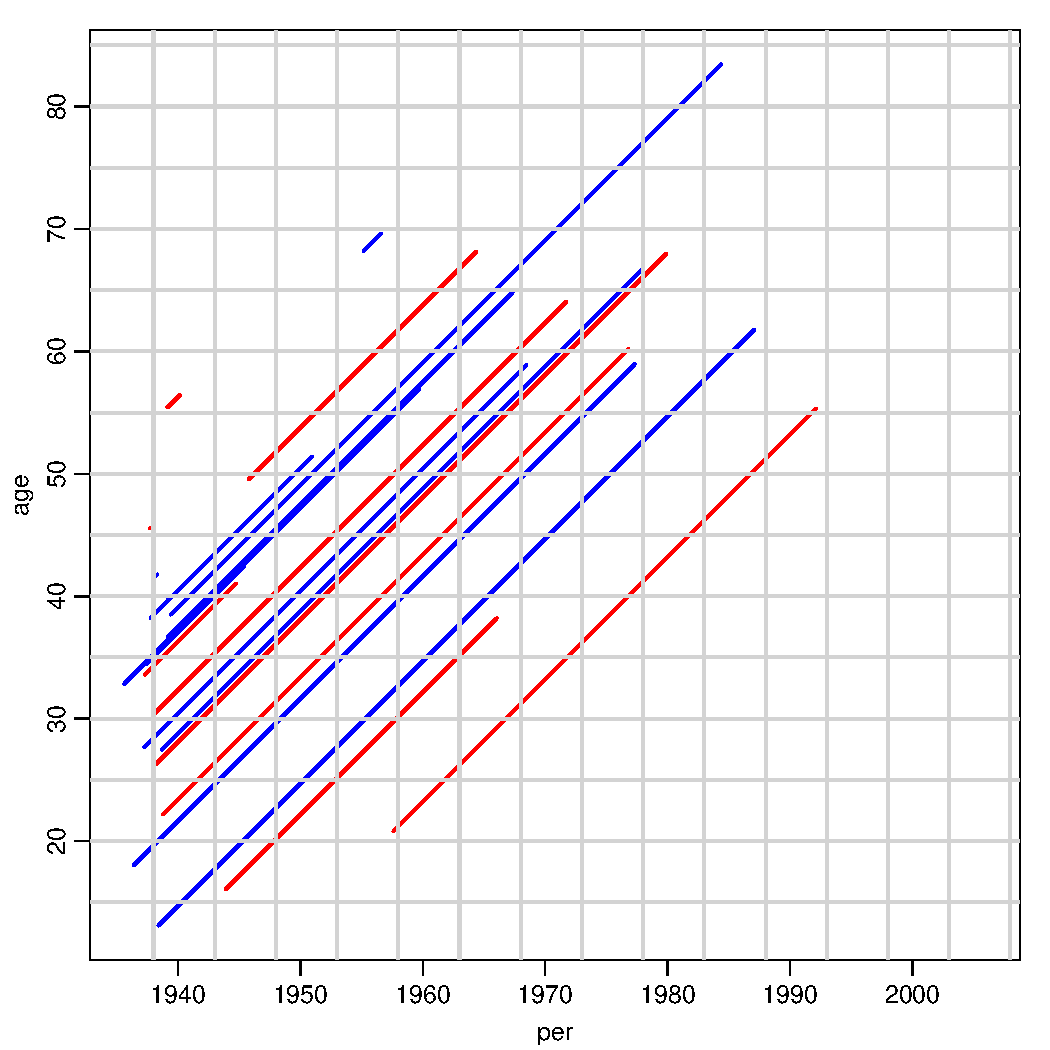
\includegraphics[height=0.99\textheight,keepaspectratio]{thL-lexis3}
\end{frame}

%----------------------------------------------------------------------
\begin{frame}[fragile]
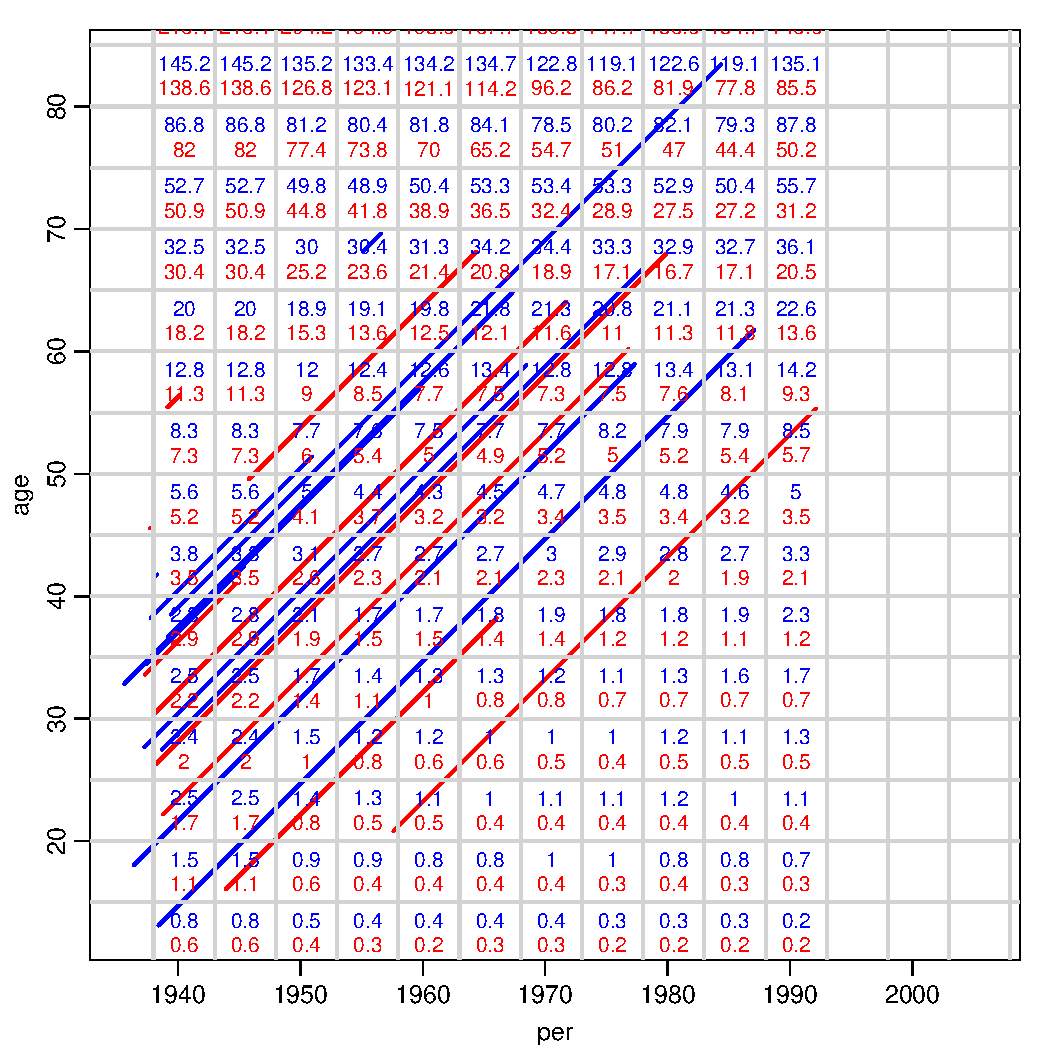
\includegraphics[height=0.99\textheight,keepaspectratio]{thL-lexis4}
\end{frame}

%----------------------------------------------------------------------
\begin{frame}[fragile]{Split the data to fit with population data}
\begin{Schunk}
\begin{Sinput}
> tha  <- splitLexis(thL, time.scale="age", breaks=seq(0,90,5) )
> thap <- splitLexis(tha, time.scale="per", breaks=seq(1938,2038,5) )
> dim( thap )
\end{Sinput}
\begin{Soutput}
[1] 23094    21
\end{Soutput}
\end{Schunk}
\pause
\vspace*{-1em}
Create variables to fit with the population data
\vspace*{-1ex}
\begin{Schunk}
\begin{Sinput}
> thap$agr <- timeBand( thap, "age", "left" )
> thap$cal <- timeBand( thap, "per", "left" )
> round( thap[1:5,c("lex.id","age","agr","per","cal","lex.dur","lex.Xst","sex")], 2 )
\end{Sinput}
\begin{Soutput}
  lex.id   age agr     per  cal lex.dur lex.Xst sex
1      1 22.18  20 1938.79 1938    2.82       0   2
2      1 25.00  25 1941.61 1938    1.39       0   2
3      1 26.39  25 1943.00 1943    3.61       0   2
4      1 30.00  30 1946.61 1943    1.39       0   2
5      1 31.39  30 1948.00 1948    3.61       0   2
\end{Soutput}
\end{Schunk}
\end{frame}

%----------------------------------------------------------------------
\begin{frame}[fragile]
\begin{Schunk}
\begin{Sinput}
> data( gmortDK )
> gmortDK[1:6,1:6]
\end{Sinput}
\begin{Soutput}
  agr per sex   risk    dt     rt
1   0  38   1 996019 14079 14.135
2   5  38   1 802334   726  0.905
3  10  38   1 753017   600  0.797
4  15  38   1 773393  1167  1.509
5  20  38   1 813882  2031  2.495
6  25  38   1 789990  1862  2.357
\end{Soutput}
\begin{Sinput}
> gmortDK$cal <- gmortDK$per+1900
> #
> thapx <- merge( thap, gmortDK[,c("agr","cal","sex","rt")] )
> #
> thapx$E <- thapx$lex.dur * thapx$rt / 1000
\end{Sinput}
\end{Schunk}
\end{frame}

%----------------------------------------------------------------------
\begin{frame}[fragile]
\begin{Schunk}
\begin{Sinput}
> stat.table( contrast,
+             list( D = sum( lex.Xst ),
+                   Y = sum( lex.dur ),
+                   E = sum( E ),
+                 SMR = ratio( lex.Xst, E ) ),
+              margin = TRUE,
+                data = thapx )
\end{Sinput}
\begin{Soutput}
 -------------------------------------------- 
 contrast         D        Y       E     SMR  
 -------------------------------------------- 
 1           923.00 20072.53  222.01    4.16  
 2          1036.00 31839.35  473.88    2.19  
                                              
 Total      1959.00 51911.87  695.89    2.82  
 -------------------------------------------- 
\end{Soutput}
\end{Schunk}
\end{frame}

%----------------------------------------------------------------------
\begin{frame}[fragile]
\begin{Schunk}
\begin{Soutput}
 -------------------------------------------- 
 contrast         D        Y       E     SMR  
 -------------------------------------------- 
 1           923.00 20072.53  222.01    4.16  
 2          1036.00 31839.35  473.88    2.19  
                                              
 Total      1959.00 51911.87  695.89    2.82  
 -------------------------------------------- 
\end{Soutput}
\end{Schunk}
\vspace*{-1em}
\begin{Schunk}
\begin{Sinput}
> m.SMR <- glm( lex.Xst ~ factor(contrast) - 1,
+               offset = log(E),
+               family = poisson, 
+                 data = thapx )
> round( ci.exp( m.SMR ), 2 )
\end{Sinput}
\begin{Soutput}
                  exp(Est.) 2.5% 97.5%
factor(contrast)1      4.16 3.90  4.43
factor(contrast)2      2.19 2.06  2.32
\end{Soutput}
\end{Schunk}
\pause
\begin{itemize}
\item Analysis of SMR is like analysis of rates:
\item Replace $Y$ with $E$ --- that's all! 
\end{itemize}
\end{frame}
